\begin{tikzpicture}
	\savebox\mygraphic{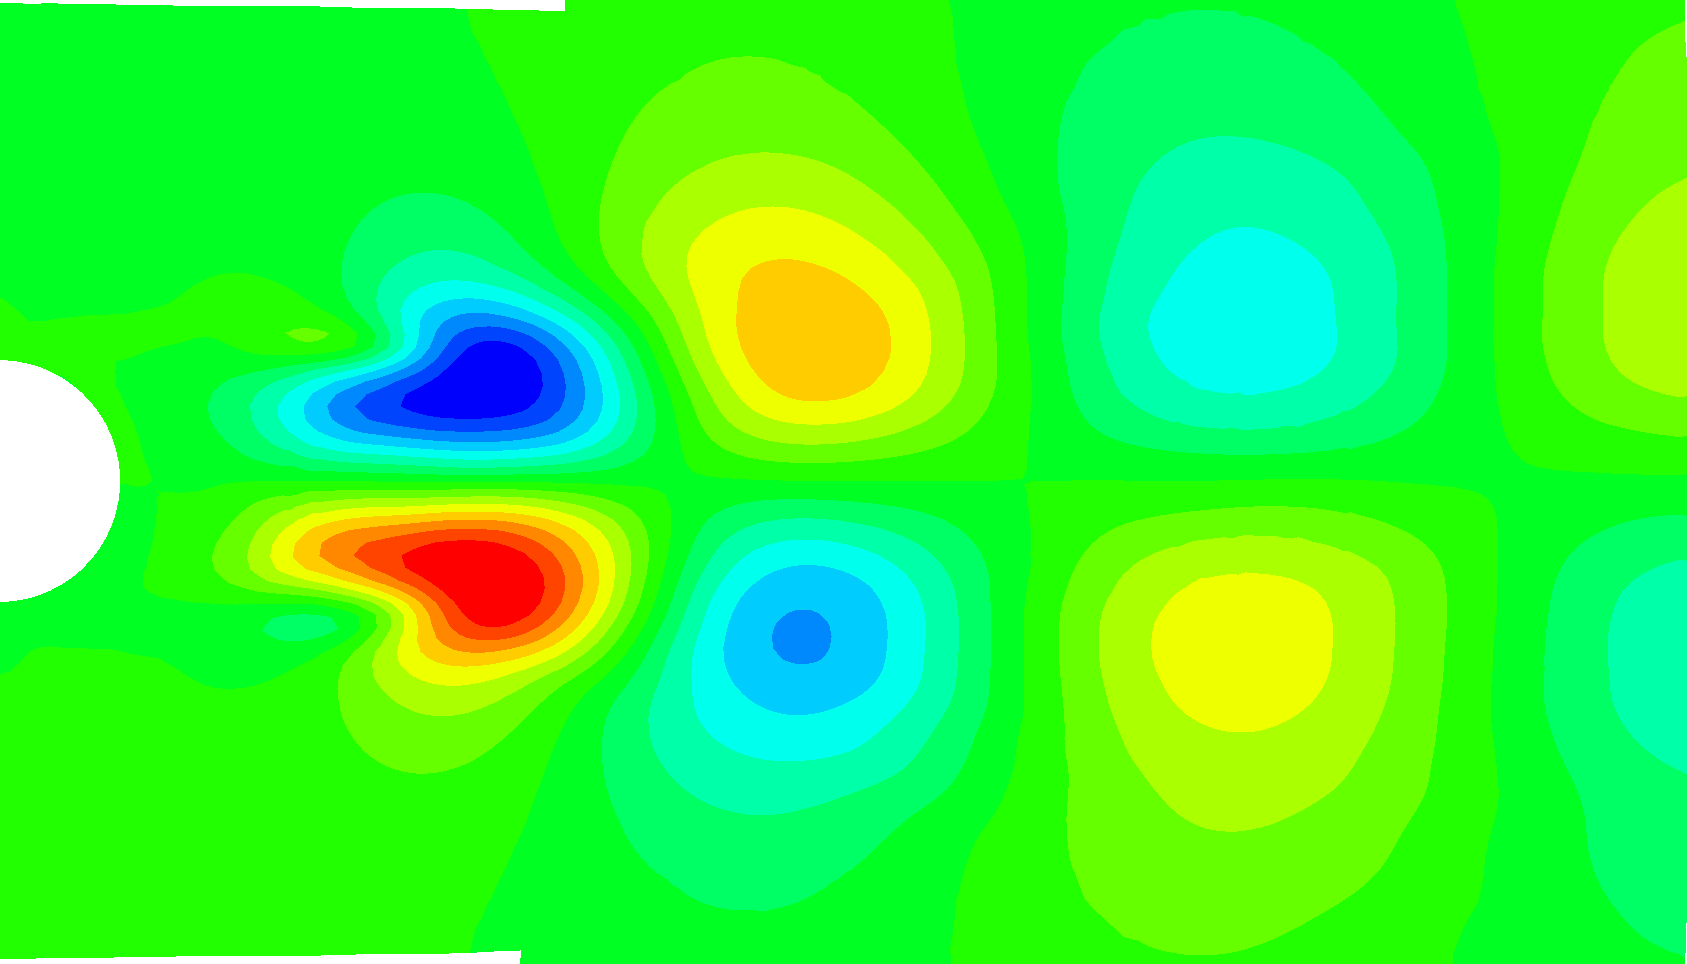
\includegraphics[trim = 0px 0px 0px 0px,clip,width = 0.39\textwidth]{\myImages/res/pom1top1numUx.png}}
	\begin{axis}[
		name = plot1,
		xlabel={$x_r$ [--]},
		ylabel={$y_r$ [--]},
		font = \scriptsize,
		xtick distance=1,ytick distance=1,
		width=\wd\mygraphic,
		height=\ht\mygraphic, %height= 5/3*0.5
		enlargelimits=false,
		scale only axis=true,
		tick align=outside,
		ytick pos=left,
		xtick pos=top,
		% x label style = {at={(axis description cs:3.5,2.5)}},
		x label style = {at={(axis cs:3.5,2.7)}},
		y label style = {at={(axis cs:-1,0)}},
		line width = 1.7pt
		]
		\addplot graphics[xmin=0, xmax=7, ymin=-2, ymax=2,includegraphics={trim = 0px 0px 0px 0px,clip}] {\myImages/res/pom1top1numUx.png};
		\fill [white] (axis cs:0.001,-1.997) rectangle (axis cs:0.5,1.997);
		\fill [black!70](axis cs:0,0) circle [radius=0.5];
		\node at (axis cs:0.22,1.7) {\scriptsize{a)}};
		% \draw [black,dashdotted,line width = 1.3pt] (axis cs:0,0) -- (axis cs:7,0);
		% \node at (axis cs:6.5,1.7) {\scriptsize{PIV}};
		% \node at (axis cs:6.5,-1.7) {\scriptsize{CFD}};
	\end{axis}

	\node [name = osaPsix,anchor = north,at={(plot1.south)},yshift=-0.1cm] {
\includegraphics[width=0.39\textwidth]{\myImages/res/psi1_x_scale.png}};
	\node [name = psi0, anchor = north,at={(osaPsix.south)},yshift=0.2cm] {\scriptsize{0}};
	\node [name = psi, anchor = north,at={(psi0.south)},yshift=0.1cm] {\scriptsize{$\bm{\psi}_{1,x},\,_{\mathrm{r}}\bm{\psi}_{1,x}$}};
	\node [name = psiM05, anchor = north west,at={(osaPsix.south west)},yshift=0.2cm] {\scriptsize{negative}};
	\node [name = psiM05, anchor = north east,at={(osaPsix.south east)},yshift=0.2cm] {\scriptsize{positive}};

	% \node [name = psiM05, anchor = center,at={(psi0.center)},xshift=-1.2cm] {positive}};

	\savebox\mygraphic{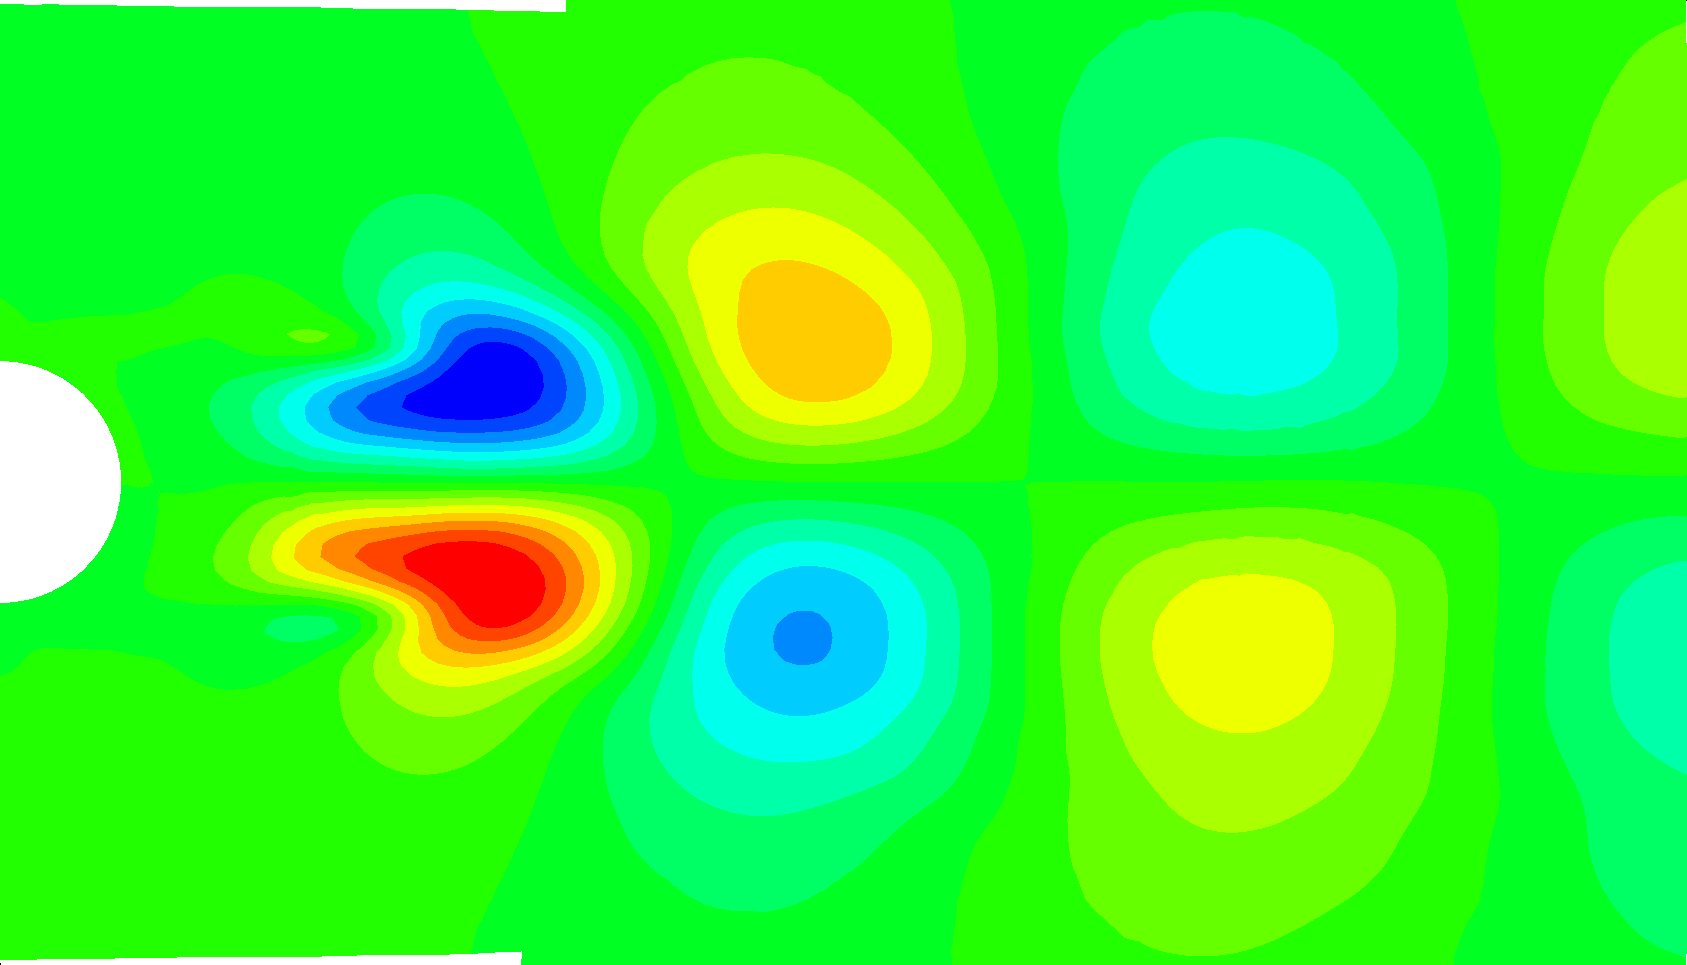
\includegraphics[trim = 0px 0px 0px 0px,clip,width = 0.39\textwidth]{\myImages/res/pom1top1numRNDpodUx.png}}
	\begin{axis}[
		name = plot2,
		anchor = north,
		at = {(psi.south)},
		yshift = -0.18cm,
		xlabel={$x_r$ [--]},
		ylabel={$y_r$ [--]},
		font = \scriptsize,
		xtick distance=1,ytick distance=1,
		x label style = {at={(axis cs:3.5,-2.7)}},
		y label style = {at={(axis cs:-1,0)}},
		width=\wd\mygraphic,
		height=\ht\mygraphic, %height= 5/3*0.5
		enlargelimits=false,
		scale only axis=true,
		ytick pos=left,
		xtick pos=bottom,
		tick align=outside,
		line width = 1.7pt
		]
		\addplot graphics[xmin=0, xmax=7, ymin=-2, ymax=2,includegraphics={trim = 0px 0px 0px 0px,clip}] {\myImages/res/pom1top1numRNDpodUx.png};
		\fill [white] (axis cs:0.001,-1.997) rectangle (axis cs:0.5,1.997);
		\fill [black!70](axis cs:0,0) circle [radius=0.5];
		\node at (axis cs:0.22,1.7) {\scriptsize{c)}};
		% \draw [black,dashdotted,line width = 1.3pt] (axis cs:0,0) -- (axis cs:7,0);
		% \node [color=white] at (axis cs:6.5,1.7) {\scriptsize{PIV}};
		% \node [color=white] at (axis cs:6.5,-1.7) {\scriptsize{CFD}};
	\end{axis}

	\savebox\mygraphic{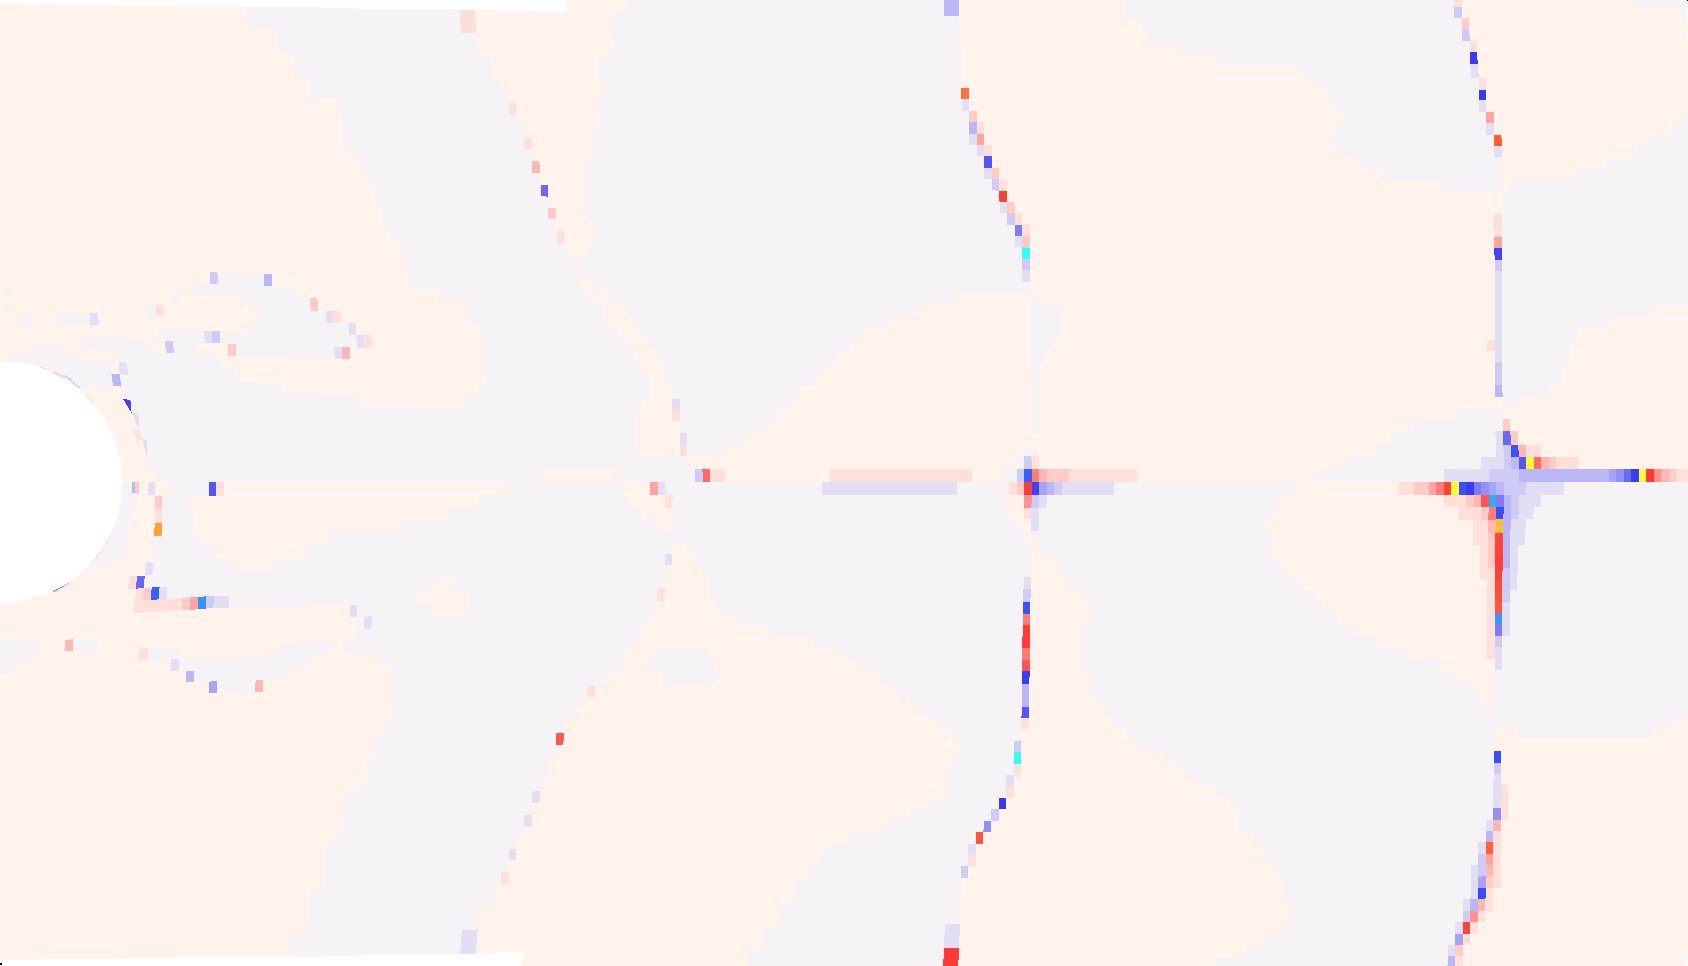
\includegraphics[trim = 0px 0px 0px 0px,clip,width = 0.39\textwidth]{\myImages/res/relDiffpodRNDpod.png}}
	\begin{axis}[
		name = plot3,
		xshift = 0.4cm,
		anchor = west,
		at = {(plot1.east)},
		xlabel={$x_r$ [--]},
		ylabel={$y_r$ [--]},
		font = \scriptsize,
		x label style = {at={(axis cs:3.5,2.7)}},
		y label style = {at={(axis cs:8,0)}},
		xtick distance=1,ytick distance=1,
		width=\wd\mygraphic,
		height=\ht\mygraphic, %height= 5/3*0.5
		enlargelimits=false,
		scale only axis=true,
		ytick pos=right,
		xtick pos=top,
		tick align=outside,
		line width = 1.7pt
		]
		\addplot graphics[xmin=0, xmax=7, ymin=-2, ymax=2,includegraphics={trim = 0px 0px 0px 0px,clip}] {\myImages/res/relDiffpodRNDpod.png};
		\fill [white] (axis cs:0.001,-1.997) rectangle (axis cs:0.5,1.997);
		\fill [black!70](axis cs:0,0) circle [radius=0.5];
		\node at (axis cs:0.22,1.7) {\scriptsize{b)}};
		% \draw [black,dashdotted,line width = 1.3pt] (axis cs:0,0) -- (axis cs:7,0);
		% \node [color=white] at (axis cs:6.5,1.7) {\scriptsize{PIV}};
		% \node [color=white] at (axis cs:6.5,-1.7) {\scriptsize{CFD}};
	\end{axis}
	
	\node [name = osaPsix,anchor = north,at={(plot3.south)},yshift=-0.1cm] {
\includegraphics[width=0.39\textwidth]{\myImages/res/relDiff_x_scale.png}};
	\node [name = psi0, anchor = north,at={(osaPsix.south)},yshift=0.2cm] {\scriptsize{0 \%}};
	\node [name = psi, anchor = north,at={(psi0.south)},yshift=0.1cm] {\scriptsize{$(\bm{\psi}_{1,x}-\,_{\mathrm{r}}\bm{\psi}_{1,x})/\bm{\psi}_{1,x}$}};
	\node [name = psiM05, anchor = north west,at={(osaPsix.south west)},yshift=0.2cm] {\scriptsize{-0.1 \%}};
	\node [name = psiM05, anchor = north east,at={(osaPsix.south east)},yshift=0.2cm] {\scriptsize{0.1 \%}};

	\begin{axis}[
		name = plot4,
		anchor = west,
		at = {(plot2.east)},
		xshift = 0.4cm,
		xlabel={mode number $j$},
		ylabel={$|\sigma_j - _{\mathrm{r}}\sigma_j|/\sigma_1$ [--]},
		font = \scriptsize,
		% xtick distance=1,ytick distance=1,
		width=\wd\mygraphic,
		height=\ht\mygraphic, %height= 5/3*0.5
		% x label style = {at={(axis cs:3.5,-2.7)}},
		% y label style = {at={(axis cs:-1,0)}},
		enlargelimits=false,
		scale only axis=true,
		ytick pos=right,
		xtick pos=bottom,
		ymode=log,
		line width = 0.85pt,
		xmax=30,
		xmin=0,
		ymin=1e-14,
		ymax=0.1,
		ytick={1e-1,1e-5,1e-10,1e-14}
		% tick align=outside,
		]
		\addplot [color = black,mark =triangle,only marks] table [x expr=\thisrow{x}+1, y expr = \thisrow{scaledWRTSigma1}]{\myGraphs/singValsData/singValsRND_U.dat};
		
		% \addplot [color = red,mark =x,only marks] table [x expr=\thisrow{x}+1, y expr = \thisrow{singVal}]{\myGraphs/singValsData/singValsRND_U.dat};
		% \addplot graphics[xmin=0, xmax=7, ymin=-2, ymax=2,includegraphics={trim = 0px 0px 0px 0px,clip}] {\myImages/res/relDiffpodRNDpod.png};
		% \fill [white] (axis cs:0.001,-1.997) rectangle (axis cs:0.5,1.997);
		% \fill [black!70](axis cs:0,0) circle [radius=0.5];
		% \draw [black,dashdotted,line width = 1.3pt] (axis cs:0,0) -- (axis cs:7,0);
		% \node [color=white] at (axis cs:6.5,1.7) {\scriptsize{PIV}};
		% \node [color=white] at (axis cs:6.5,-1.7) {\scriptsize{CFD}};
	\end{axis}
	\node[anchor=north west] at (plot4.north west) {\scriptsize{d)}};
\end{tikzpicture}
